\chapter{Testing}
\label{chap:testing}
\textit{This chapter presents the results of unit testing and our discussion on security perspectives. Section \ref{testlib} describes our works on the open-source library, and Section \ref{testhd} evaluates the non-custodial HD wallet.}

\minitoc

\section{The Library}
\label{testlib}
\subsection{Testcases}

We run a total of 10 test cases to make sure every API functions normally according to its definition (presenting tests with Solana and ed25519 keys). 

\bigskip
{\textbf{Test data}}

\begin{framed}
    \hspace*{13mm}        \{ \par
    \hspace*{13mm}        "mnemonic" : 'honey opera much plate gloom accuse honey pudding chase beach flight pencil velvet apart series pepper antenna hill amazing season foot goddess harsh theory',    \par
    \hspace*{13mm}        "master\_seed" : 'd51741549ced8fdce60e30ff8c0b885d6f156dfc44 \par
    \hspace*{27mm}         b7de53dc66b5f8c3a3d48e06b1fd7c8c8c73748e2e78db3f84a4ba \par
    \hspace*{27mm}         e855c9304e14f593674870a1db5cdb6d',    \par
    \hspace*{13mm}        "m\/44'\/501'\/0'\/0'\/10'" : 'HSPjBD1z \par
    \hspace*{37mm}        JLgj29hy8i7DD4HmaDPDh3bc1N2J4Dx9qsRn' \par
    \hspace*{13mm}              \} \par
    \end{framed}

\bigskip
{\textbf{Test table}}
\bigskip

\begin{tabular}{ m{2cm} m{6cm}  m{2cm}  m{3cm}  m{2cm} }
    \toprule
    ID & Description & Expected Result & Actual Result & Pass/Fail                                            \\ 
    \midrule
    SOL-01 & Generate a valid mnemonic code contains 12 or 24 words. & Generate successfully & As expected & Pass \\ 
    SOL-02 & Generate a valid master secret seed.  &  Generate successfully & As expected & Pass  \\ 
    SOL-03 & Generate a valid master key pair. &   Generate successfully & As expected & Pass    \\ 
    SOL-04 & Generate a valid path. &  Generate successfully & As expected & Pass   \\ 
    SOL-05 & Generate a valid child key pair. &  Generate successfully & As expected & Pass   \\ 
    SOL-06 & Generate a valid public address.&  Generate successfully & As expected & Pass   \\ 
    SOL-07 & Generate a child generated from given mnemonic.&  Generate successfully & As expected & Pass   \\
    \bottomrule
\end{tabular}
% \captionof{table}{\label{Tab:SOL-01} Library testcases}

\bigskip
{\textbf{Test with mocha (Javascript testing framework)}}

\bigskip
\autoref{fig:testmocha} presents the results of mocha framework testing for our library.
\bigskip

\begin{figure}[ht!]
    \centering
    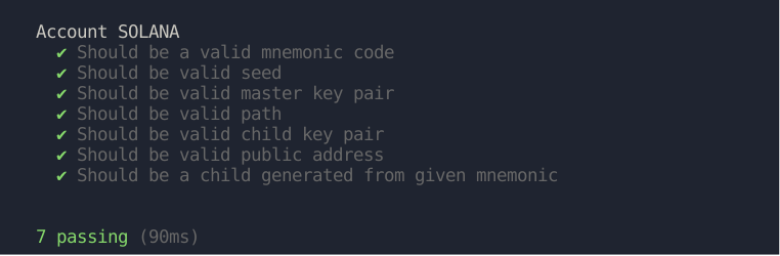
\includegraphics[width=1\textwidth]{images/test_mocha.png}
    \caption[Testcase results with mocha]{Testcase results with mocha}
    \label{fig:testmocha}
\end{figure}

We tested the HD key tree generation with mocha. The transaction between wallets is a bit hard to confirm the result, so we use Jupyter Notebook instead.

\bigskip
{\textbf{Test with mocha (Javascript testing framework)}}
\bigskip

We import Nodejs kernel to notebook environment and start a session. The grey part is a cell to input code. Below every cell is result of code compilation.

\begin{itemize}
    \item Test airdrop (see \autoref{fig:testairdrop}).
    \item Checking the address balance (see \autoref{fig:testbalance}).
    \item Sending 0.05 SOL to another address (see \autoref{fig:testtransaction}).
    \item Checking the return transaction hash on Solana Explorer (see \autoref{fig:testexpl1} and \autoref{fig:testexpl2}).Solana Explorer is a website to look up transactions and accounts on the various Solana clusters. In Figure. We can see we transferred 0.05 SOL as the instruction in the notebook Figures.

    \begin{figure}[ht!]
        \centering
        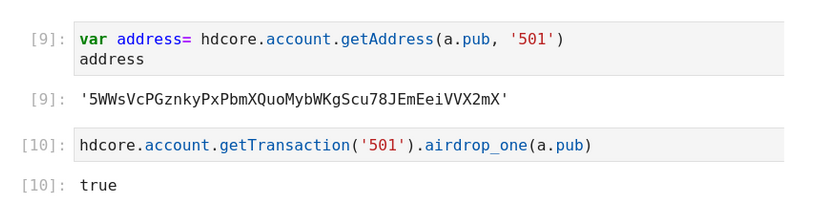
\includegraphics[width=1\textwidth]{images/testairdrop.png}
        \caption[Test airdrop with Solana]{Test airdrop with Solana}
        \label{fig:testairdrop}
    \end{figure}
    \begin{figure}[ht!]
        \centering
        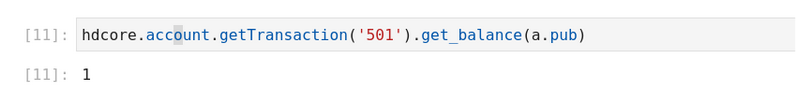
\includegraphics[width=1\textwidth]{images/testgetbalance.png}
        \caption[Test balance with Solana]{Test balance with Solana}
        \label{fig:testbalance}
    \end{figure}
    \begin{figure}[ht!]
        \centering
        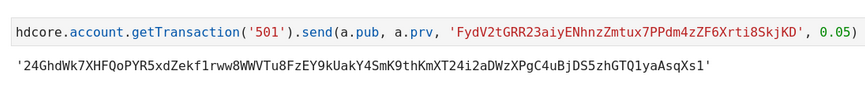
\includegraphics[width=1\textwidth]{images/testtransaction.png}
        \caption[Test transaction with Solana]{Test transaction with Solana}
        \label{fig:testtransaction}
    \end{figure}

    \begin{figure}[ht!]
        \centering
        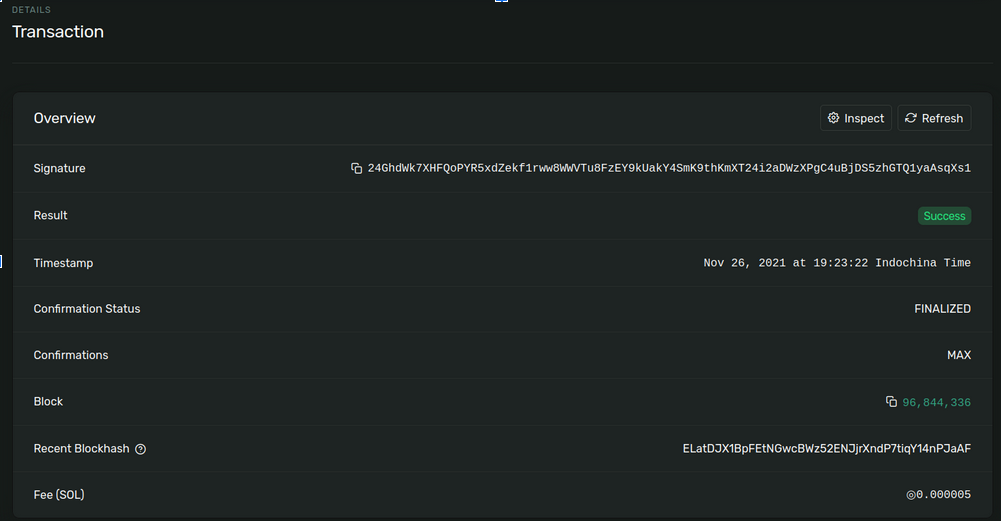
\includegraphics[width=1\textwidth]{images/testexplore1.png}
        \caption[Transaction detail on Solana Explorer]{Transaction detail on Solana Explorer}
        \label{fig:testexpl1}
    \end{figure}

    \begin{figure}[ht!]
        \centering
        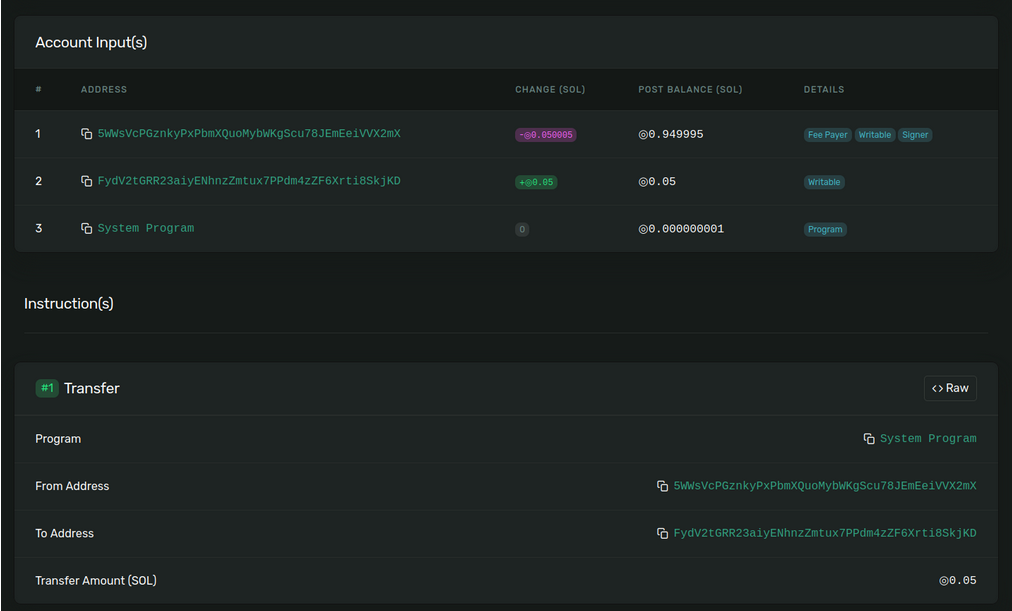
\includegraphics[width=1\textwidth]{images/testexplorer2.png}
        \caption[Coins transfered details]{Coins transfered details}
        \label{fig:testexpl2}
    \end{figure}

\end{itemize}

\subsection{Security Discussion}

We acknowledge that cryptography is a tool to achieve security. Still, if we get anything wrong in the cryptography implementation, that will not deliver the protection it was meant to offer, and it will become ineffective. We focused on researching the security flaws as the warning in the proposed paper to avoid implementing bad crypto.

Digital signature generation libraries like tweetnacl and secp256k1 (for Solana and Ethereum keys) are completely free of timing side-channels since they provide constant time and constant memory access. We look into their publication and implementation to observe their approach compared to the original paper.

We use the hardened key derivation schema of the BIP32 and SLIP10 to avoid the key recovery attack on public key derivation because our wallet is a hot wallet type. We examine the potential vulnerabilities of the BIP32-ED25519 paper for ed25519 curves and take the researcher's recommendation seriously. To compensate for the inconvenience of hardened key schema, we created a system alongside our library to provide a comfortable assets exchange.

We also make sure the requests and connection of the wallet to the blockchain will not leak any important information about the created wallet. Overall, our library applied a provable cryptography library and followed the safest schema in the industrial community, and improvised the efficiency by current technology.

\section{The Hierarchical Deterministic Web Wallet}
\label{testhd}
\subsection{Testcases}
We test our Web Wallet behaviors by following testcases.

{\textbf{Test table}}

\begin{tabular}{ m{1.5cm} m{4.5cm} m{5cm} m{3cm} m{1.5cm}}
    \toprule
    ID & Description & Expected Result & Actual Result & Pass/Fail                                            \\ 
    \midrule
    HDW-01 & Create a new mnemonic word and create a new wallet from it. & Go to the main page successfully & As expected & Pass \\ 
    HDW-02 & Import a mnemonic word and restore a wallet.  &  Go to the main page successfully. & As expected & Pass  \\ 
    HDW-03 & Request airdrop 1 SOL from the Solana devnet. &  The balance increased by 1 SOL. & As expected & Pass    \\ 
    HDW-04 & Transfer 0.05 SOL using send in the main page. &  The balance is reduced by the 0.05 SOL with some fee (0.00005 SOL), and the receiver received 0.05 of SOL & As expected & Pass   \\ 
    HDW-05 & Delete and logout in the main page. &  The localStorage is cleared and the user is brought to the homepage. & As expected & Pass   \\ 
    HDW-06 & Push a child address to the address service.&  The server received the request and store the address to the database. & As expected & Pass   \\ 
    HDW-07 & Pull a child address from the address service.&  The server received the request and delete the address from the database. & As expected & Pass   \\ 
    HDW-08 & Create a child wallet in the main page.&  A wallet is create with the path includes the index provided by the user and the purpose is displayed correctly from the user's input. & As expected & Pass   \\ 
    HDW-09 & Search a child wallet's address using the master wallet address in the main page.& Display all the pushed child wallets's addresses of the master address from the databases. & As expected & Pass   \\ 
    \bottomrule
\end{tabular}
\subsection{Security Discussion}

We think that no system is perfectly safe from security threats. At least, we can prevent common attacks from happening. Observing mentioned OWASP’s securities risk, we present as follows:

\begin{itemize}
    \item \textbf{Broken Access Control}.
    \begin{quote}
        The Address service is highly vulnerable to this attack since we design it with no authentication at all. Access control enforces policy such that users cannot act outside of their intended permissions. No authentication lead to an attacker can poison other address databases. For example, they can push their addresses into each other documents in MongoDB and impersonate their child addresses. However, we consider this vulnerability is deemed to be easy to solve. In this thesis, we created a demo product. In practice, we could avoid this attack for our service with any server we deployed on with a regular authentication token for each user.
    \end{quote}
    \item \textbf{Cryptographic Failures}.
    \begin{quote}
        Our web wallet security depends on heavy cryptography. We created a library that takes parts as a core of our fundamental cryptography to prevent this vulnerability. The provable security of our library is discussed in Section \ref{testlib}.
    \end{quote}
    \item \textbf{Injection}.
    \begin{quote}
        We prevent injection attacks by carefully checking the user’s input and rejecting them if they belong to scripts group.
    \end{quote}
    \item \textbf{Insecure Design}.
    \begin{quote}
        Secure design is a culture and methodology that constantly evaluates threats and ensures that code is robustly designed and tested to prevent known attack methods. We designed a system that leaks no sensitive information of the user. We also researched well-concerned attack vectors on our system and the library and prevented it in our implementation.    \end{quote}
    \item \textbf{Vulnerable and Outdated Components}.
    \begin{quote}
        Library and frameworks we used are up-to-date and well researched. We removed all unnecessary features, components, and samples. There are no redundant or risks contained in the library that we applied.
    \end{quote}
\end{itemize}
In conclusion, we covered famous attacks on standard web applications and ran test cases for the software to behave appropriately. There are some potential attacks on the client-side that we (the service provider) cant handle. Where users access some malicious software, log in their mnemonic seeds to the wrong website, etc.

